\documentclass[../main.tex]{subfiles}
\begin{document}
\setchapterstyle{kao}
\setchapterpreamble[u]{\margintoc}
\chapter[Tool: Polar decomposition]{Tool: Polar decomposition\footnotemark[0]}
\labch{too-pol-dec}
This is a tool which will be useful later, we will use the decomposition for matrices, but actually the same theory, with more or less the same proofs, also works for bounded operators in Hilbert spaces.
\section{Introduction}
The polar decomposition for numbers is something we are already familiar with: a complex number $z\in\mathbb{C}$, with $z$ invertible (which means $z\neq 0$ for numbers) can be decomposed in the polar form:\marginnote[5mm]{Usually it is used the greek letter $\rho$, but \textbf{P}anati uses $P$ to remind himself that it is \textbf{P}ositive}
\[
z=e^{i\overset{\mathclap{\tikz \node {$\downarrow$} node [above=1.25ex] {\footnotesize not unique!$\ $};}}{\theta}}P=\underset{\mathclap{\tikz \node {$\uparrow$} node [below=1ex] {\footnotesize \text{\parbox{3 cm}{\centering unimodular\\[-3pt] $u\in\textrm{U}(1)$}}};}}{u}\overset{\mathclap{\tikz \node {$\downarrow$} node [above=1.25ex] {\footnotesize $\ $ positive};}}{P}=ue^x
\]
where $\theta$ is called \textit{phase}. \begin{marginfigure}
	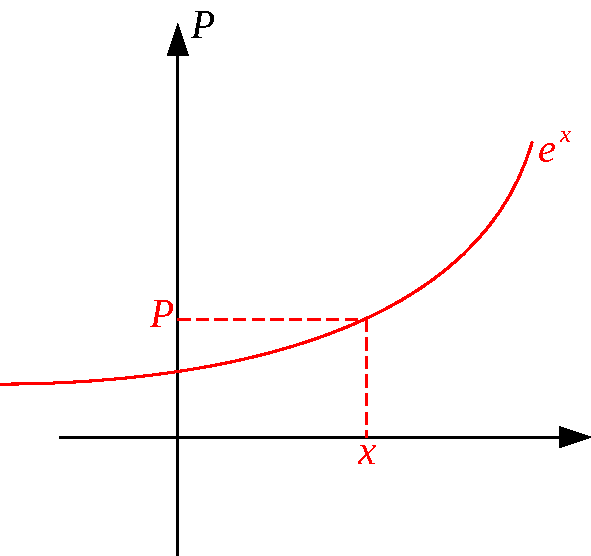
\includegraphics[width=1\linewidth]{images/polar_dec.pdf}
	\caption{Polar decomposition of a number/matrix using exponential since the map is bijective.}
	\labfig{pol-dec}
\end{marginfigure}The first part is the usual way that is in every book, but this does \textbf{not} work well for matrices, because $\theta$ is not unique! It is defined with an ambiguity of $\abs{2\pi n}, n\in\mathbb{Z}$; while for numbers this is more or less acceptable, if we do the same for matrices, we will have an ambiguity of $\abs{2\pi n}$ on each eigenvalue: $\abs{2\pi n}^N$ + interference between different eigenvalues, this would be a nightmare. Therefore we prefer to write the polar decomposition using unimodular numbers (complex numbers of modulus one, so a point in the circle) times a real number, therefore there is no ambiguity on the phase. But a positive number can be written uniquely as the exponential of a real number, because the exponential is bijective from $\mathbb{R}$ to $[0,+\infty)$. We are simply saying that a positive real number $P$ can be written uniquely as the exponential for some $x$, as in \reffig{pol-dec}, since the map is bijective.

Notice that the decomposition we wrote for numbers works well, if $z\neq 0$, otherwise for $z=0$ the modulus is still zero, but the phase is undefined. This condition for operators will be not only different form zero, but invertible (the two things coincide for numbers).

As far as numbers are concerned, we can harmless switch from one way of writing to the other (provided that we remember that $\theta$ is defined up to $2\pi n$), but for matrices we will take the form $uP$. Nevertheless, firstly we have to say what is a positive matrix, and therefore a positive operator.
\begin{definition}[Positive operator]\index{Positive operator} A \textbf{positive} linear operator acting on $\mathcal{H}=\mathbb{C}^n$ is a \textbf{self-adjoint}\marginnote{If it is self-adjoint, the spectrum is real} operator such that all the matrix elements are positive
\begin{equation}\labeq{pos-oper}
(\star) \qquad \braket{v}{Pw}>0 \qquad \forall v,w\in\mathbb{C}^n
\end{equation}
where $\langle \dots,\; \dots\rangle$ is the usual inner product in $\mathbb{C}^n$.
\[
\langle z,\;w\rangle = \sum_{j=1}^n\overline{z}_jw_j
\]
As $\dim(\mathbb{C}^n)=n<+\infty$, then (\ref{eq:pos-oper}) is equivalent to the fact the \textbf{all the eigenvalues $\lambda_j$ of $P$ are positive ($\star \star$).}
\end{definition}
\section{Main result}
Once we know what is a positive operator, we can hope to generalize the polar decomposition of a complex number into something similar for operators: the analogous of a positive number will be a positive operator and the analogous of unimodular numbers will be a unitary operator, which is the natural generalization since it has all the eigenvalues on the complex circle.
\begin{theorem}[Polar decomposition - general]\index{Polar decomposition - general}\labthm{pol-dec-gen} It holds true that:
\renewcommand{\labelenumi}{\arabic{enumi})}
\begin{enumerate}
    \item Every $A\in\textrm{GL}(n,\mathbb{C})$ can be written \underline{\textbf{uniquely}} as\marginnote{With positive we mean already self-adjoint and positive} 
    \[
    A=UP \quad \begin{cases}
    P \quad \textrm{positive}\\
    U \quad \textrm{unitary}
    \end{cases}
    \]
    \item Every $P^\ast=P>0$ \textbf{(positive!)} can be written \underline{\textbf{uniquely}} as
    \[
    P=e^X \qquad X^\ast=X
    \]
\end{enumerate}
Putting the two pieces together
\renewcommand{\labelenumi}{3)}
\begin{enumerate}
    \item If we decompose an invertible matrix $A\in\textrm{GL}(n,\mathbb{C})$ \textbf{uniquely} as
    \[
    A=Ue^X \quad \begin{cases}
    U \quad \textrm{unitary}\\
    X \quad \textrm{self-adjoint}
    \end{cases}
    \]
    then the maps $ A \mapsto U$ and $A\mapsto X$ are \textbf{continuous} (and rather explicit!)\marginnote{It is so explicit, that the proof will not be exhibited for these maps}
\end{enumerate}
\end{theorem}
\section{Square root lemma}
We already had a square root lemma (\reflemma{loc-square-root}), but in a different sense, this is the square root for self-adjoint operators. Let us emphasize that in general, the square root of an operator, even invertible $A\in\textrm{GL}(n,\mathbb{C})$, is not unique.
\begin{example}
Let us take the $2\times 2$ identity and let us look for the square roots:
\[
A=\begin{pmatrix}
1 & 0\\
0 & 1
\end{pmatrix}=B^2 \quad \Rightarrow \quad B=\begin{cases}
\begin{pmatrix}
1 & 0\\
0 & 1
\end{pmatrix}\\
\begin{pmatrix}
0 & 1\\
-1 & 0
\end{pmatrix}\\
\begin{pmatrix}
0 & -1\\
1 & 0
\end{pmatrix}\\
\vdots
\end{cases}
\]
Some of them are self-adjoint and some of them are not.
\end{example}
The fact that in general there are many square roots is bad, but is also good. It is good because otherwise there would be no Dirac equation: the Dirac operator is a non-trivial square root of the wave operator.

In some spacial cases the square root is unique: we have already seen with the \reflemma{loc-square-root} that if we are sufficiently close to zero (or respectively to the identity), the exponential and logarithm are both bijective and so we can define the square root as one-half the exponential of $a$. Now we see another special case.
\begin{lemma}\lablemma{self-pos-uni-sq-root}
If $Q=Q^\ast$ is \underline{\textbf{positive}}, then there exists a \underline{\textbf{unique}} \underline{\textbf{positive}} \textbf{square root}
\end{lemma}
\begin{proof}
$Q=Q^\ast$ is ortho-diagonalizable (via an ortho-nomral basis, or unitary matrix if you prefer), i.e. $\exists$ a unitary $U$ such that $Q$ is similar via $U$ to a diagonal matrix:
\[
Q=U\;\begin{pmatrix}
\lambda_1 & & 0\\
 & \ddots & \\
0 & &\lambda_n
\end{pmatrix}\;U^{-1}
\]
As $Q>0$ each eigenvalue satisfies\marginnote{This is the little part which will not work in infinite dimension and it should be adapted. Usually in mathematics, natural things are also correct. Of course, you have to check that they are correct, but to do something natural, in a sense, is the good thing} $\lambda_j>0$, the only natural way to define the square root is:
\[
\sqrt{Q}:=U\;\begin{pmatrix}
\sqrt{\lambda_1} & & 0\\
 & \ddots & \\
0 &  &\sqrt{\lambda_n}
\end{pmatrix}\;U^{-1} \qquad \Big|\Big| \quad \star
\]
% \marginnote{Usually in mathematics, natural things are also correct. Of course, you have to check that they are correct, but to do something natural in a sense is the good thing}
\underline{Check:}
\[
\left(\sqrt{Q}\right)^2=U\left(\sqrt{\lambda_j}\right)\overbrace{U^{-1}U}^{{\color{red}=\mathbb{1}}}\left(\sqrt{\lambda_j}\right)U=U\;\begin{pmatrix}
\lambda_1 & & 0\\
 & \ddots & \\
0 &  &\lambda_n
\end{pmatrix}\;U^{-1}=Q
\]
since if we multiply two diagonal matrices, we still get a diagonal matrix. It remains to prove that it is unique.

\underline{Uniqueness:} suppose $P^\ast=P>0$. Since it is self-adjoint it has a complete ortho-normal basis of eigenvectors with positive eigenvalues $p_j$\begin{marginfigure}
	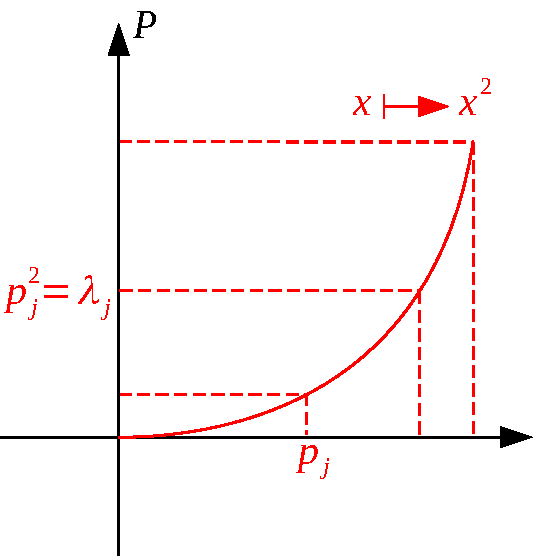
\includegraphics[width=1\linewidth]{images/uniq_polar_dec.pdf}
	\caption{Map $x\mapsto x^2$.}
	\labfig{uniq-pol-dec}
\end{marginfigure}
\[
\begin{split}
Pe_j&=p_je_j\\
P^2e_j&=\left(p_j\right)^2e_j
\end{split}
\]
So $P^2$ has the same eigenvectors as $P$. We discovered that $P^2$ is diagonalized via the same orthonormal basis as $P$: $\left\{e_1,\dots,e_n\right\}$, but with different \textbf{eigenvalues} $\lambda_j=\left(p_j\right)^2$. With the same reasoning, observing that $x\mapsto \sqrt{x}$ \textbf{is bijective on} $\left(0,+\infty\right)$, we get that $\sqrt{Q}$ is unique (\reffig{uniq-pol-dec}).
\end{proof}
What is the general moral? 
\begin{itemize}
    \item The square root of an operator is not unique, and this is a good thing (as Dirac understood).
    \item Sometimes it is unique, if we are sufficiently close to zero (even non-self-adjoint), thanks to the magic number $\log(2)$.
    \item It is also unique if we have an operator which is positive.
\end{itemize}
Now we are ready to prove the main theorem. 
\begin{proof} \textit{of \refthm{pol-dec-gen}:}
\renewcommand{\labelenumi}{\arabic{enumi})}
\begin{enumerate}
    \item We want to prove that $A=UP$.\marginnote{It is convenient to start with uniqueness, because it suggests a good definition}
    
    \underline{Uniqueness:} Suppose it is true: $A=UP$. If it is true, then:
    \[
    A^\ast A =\left(UP\right)^\ast UP=PU^\ast UP = P^2
    \]
    Very good, this already suggests what $P$ should be, it should be the square root of $A^\ast A$. As soon as we will prove that $A^\ast A$ is positive, there is a unique square root and we are done. Therefore, if such a decomposition exists, it also holds that $U=AP^{-1}$, as $P>0$ is invertible.
    
    \underline{Existence:} we have to check that $\forall\;A: \, A^\ast A$ is self-adjoint. But if $A$ is invertible $A\in\textrm{GL}(n,\mathbb{C})$ (we are using this hypotesis), then $A^\ast A$ is positive:
    \[
    \braket{v}{A^\ast Av}=\braket{Av}{Av}=\norm{Av}^2 \geq 0
    \]
    If it happens that $\norm{Av}=0$, then $Av=0$, against the fact that $A\in\textrm{GL}(n,\mathbb{C})$. Hence $A^\ast A$ is \underline{\textbf{positive!}} Then our \reflemma{self-pos-uni-sq-root} tells us that
    \[
    \begin{split}
    {\color{red}P}&{\color{red}:=\sqrt{A^\ast A}} \qquad {\color{red}\textrm{Positive}}\\
    {\color{red}U}&{\color{red}=A P^{-1}}
    \end{split}
    \]
    With $P$ we are ok, we have to check that the second line is a unitary operator, but this is easy.
    
    Check that $U$ is unitary: $U^\ast U = \mathbb{1}$?\marginnote{In finite dimension, if $U^\ast U = \mathbb{1} \ \Rightarrow \ UU^\ast = \mathbb{1}$}
    \[
    U^\ast U = \left(AP^{-1}\right)^\ast AP^{-1}\underset{\mathclap{\tikz \node {$\uparrow$} node [below=1ex] {\footnotesize  $P=\left(A^\ast A\right)^{1/2} \ \Rightarrow \ P^{-1}=\left(A^\ast A\right)^{-1/2}$};}}{=}\left(A^\ast A\right)^{-1/2}A^\ast A\left(A^\ast A\right)^{-1/2}=\mathbb{1}
    \]
    These are functions of the same self-adjoint operator, which is $A^\ast A=: B$ then $B^{-1/2}BB^{-1/2}=\mathbb{1}$.
    \item We have to prove that $P=e^X$ with $X^\ast=X$.
    
    As $P^\ast = P>0$, we know that $\exists\;U$ such that:
    \[
    {\color{red}\log}P=U\;\begin{pmatrix}
    {\color{red}\log}\lambda_1 & & 0\\
     & \ddots & \\
    0 &  &{\color{red}\log}\lambda_n
    \end{pmatrix}\;U^{-1}
    \]
    We could ask ourselves: is the logarithm defined this way the same as the one defined with power series? Well, if we are not too far from the identity $\norm{P-\mathbb{1}}<1$ (i.e. $0<\lambda_j<2$), then $\log P$ defined above (via \textbf{diagonalization}) agrees with the logarithm defined before (\vrefdef{matrix-log}, via \textbf{power-series}) and we are done by setting $X=\log P$, and then the exponential of the logarithm will be itself. But we promised the result for every self-adjoint, not only between $0$ and $2$!
    
    If $\norm{P-\mathbb{1}}\geq 1$ then: choose a large real number $a>1$ (we should take it $a\gg 1$), then we might think that, tautologically
    \[
    P=\overbrace{e^a}^{\textrm{number}}\underbrace{e^{-a}P}_{\textrm{small}} \qquad \Big|\Big| \quad \textrm{Trick!}
    \]
    since a number commutes with everything, the idea is \textit{\href{https://it.wikipedia.org/wiki/Divide_et_impera}{Dīvĭdĕ et ĭmpĕrā} - separate your enemies}: 
    \begin{itemize}
        \item one enemy is the fact that the norm of $P$ is large, but we separate this by transferring it to the exponential of $e$, which will be large, but scalar, so commutes with everything;
        \item on the other side we will have the exponential of minus $a$ times $P$, which is a matrix, but it is small.
    \end{itemize}
    Take $a>1$ so large that $\norm{e^{-a}P-\mathbb{1}}<1$\marginnote{We could also say $<\varepsilon$ for $a$ sufficiently large}. Here the logarithm is well-behaved, and then we define:
    \[
    {\color{red}X=a\mathbb{1}+\log(e^{-a}P)} \qquad \Big|\Big|
    \]
    Now we are done because in general the exponential of a sum is not the product of the exponential, but if the two operators commute, it is.\marginnote{The identity commutes with everything}
    \[
    e^X=e^{a\mathbb{1}}\cdot e^{\log(e^{-a}P)}=e^{a}\mathbb{1}e^{-a}P=P \qquad \textrm{ok \checkmark} 
    \]
    \item Continuity:\marginnote{We will just give a sketch} from explicit expressions, we know, for example, the map
    \[
    \begin{split}
    A&\mapsto \sqrt{A^\ast{\color{red}\cdot} A}=P\\
    U&\mapsto A\left(\left(A^\ast{\color{red}\cdot} A\right)^{\frac{1}{2}}\right)^{{\color{red}-1}}
    \end{split}
    \]
    The only thing that might be problematic is the inversion, but the \textbf{inversion} and \textbf{product} are continuous as far as we remain in any Lie group, e.g. in $\textrm{GL}(n,\mathbb{C})$.\marginnote{The only missing part is to check that the adjoint is continuous, but this you can check it by yourself}
\end{enumerate}
\end{proof}
\begin{kaobox}[frametitle=Remark]
The fact that we have these formulae\marginnote{\href{https://www.oxfordlearnersdictionaries.com/definition/english/formula}{The word \textbf{Formulae}, instead of \textit{formulas}, is used especially in scientific language}}
\[
\begin{split}
    &\\
    P&=\sqrt{A^\ast A}\\
    U&= A\left(A^\ast A\right)^{1/2}
\end{split} \quad\left|\quad
\begin{split}
    \textrm{Complex }&\textrm{numbers}\\
    \rho&=\left(\overline{z}z\right)^{1/2}\\
    (e^{i\theta}=)u &=\frac{z}{\left(\overline{z}z\right)^{1/2}} 
\end{split}
\right.
\]
\end{kaobox}
\end{document}
%41 min